\documentclass[answers]{exam}

\usepackage{color} 
\usepackage[table,svgnames]{xcolor}
\usepackage{lstautogobble, listings} 

\usepackage{tikz}
\usepackage{float}

\usetikzlibrary{automata, positioning, arrows}

\definecolor{bluekeywords}{rgb}{0.13, 0.19, 0.7}
\definecolor{goldenkeywords}{rgb}{0.67, 0.58, 0.13}
\definecolor{greencomments}{rgb}{0.1, 0.5, 0.2}
\definecolor{redstrings}{rgb}{0.8, 0.15, 0.1}
\definecolor{graynumbers}{rgb}{0.5, 0.5, 0.5}
\definecolor{subtlegray}{rgb}{0.98, 0.98, 0.98}

\lstset{
    autogobble,    
    columns=fullflexible,
    showspaces=false,
    showtabs=false,
    breaklines=true,
    showstringspaces=false,
    numbers=left,
    breakatwhitespace=true,
    escapeinside={(*@}{@*)},
    rulecolor=\color{lightgray},
    backgroundcolor=\color{subtlegray},
    commentstyle=\color{greencomments},
    keywordstyle=\color{bluekeywords},
    ndkeywordstyle=\color{goldenkeywords},
    stringstyle=\color{redstrings},
    numberstyle=\color{graynumbers},
    basicstyle=\ttfamily\linespread{1.15}\footnotesize,
    frame=tb,
    framesep=12pt,
    framexleftmargin=12pt,
    tabsize=4,
    captionpos=b
}

\lstdefinelanguage{TML}{ 
    keywords={changeto, move, goto, if, switch, while, module, accept, reject, halt, alphabet},
    ndkeywords={left, right, tapehead, blank},
    sensitive=true,
    comment=[l]{//},
    morecomment=[s]{/*}{*/},
    morestring=[b]',
    morestring=[b]"
}


\title{TML Worksheet}
\author{Student No: \texttt{\_\_\_\_\_\_\_\_\_\_\_\_}}

\begin{document}
    \maketitle

    \section{Writing TML Programs}
    In this section, you will be tested on writing TML programs. Three programs are given below as examples:
    \begin{itemize}
        \item \texttt{isDiv2}:
\begin{lstlisting}[language=TML]
// checks whether a binary number is divisible by 2
alphabet = {0, 1}
module isDiv2 {
    while 0, 1 {
        move right
    } if blank {
        move left
        if 0 {
            accept
        } if 1, blank {
            reject
        }
    }
}
\end{lstlisting}
        
        \item \texttt{isDiv2Rec}:
\begin{lstlisting}[language=TML]
// checks whether a binary number is divisible by 2 recursively
alphabet = {0, 1}
module isDiv2 {
    if 0, 1 {
        move right
        goto isDiv2
    } if blank {
        move left
        if 0 {
            accept
        } if 1, blank {
            reject
        }
    }
}
\end{lstlisting}
        \newpage
        
        \item \texttt{aNbN}:
\begin{lstlisting}[language=TML]
// checks whether the input is blank or of the form ab, aabb, aaabbb, etc.
alphabet = {a, b}
module aNbN {
    if blank {
        accept
    } 
    // cannot start with a b
    if b {
        reject
    } if a {
        changeto blank
        move right
        // go to the end
        while a, b {
            move right
        } 
        if blank {
            move left
            // must end with a b
            if a, blank {
                reject
            } if b {
                changeto blank
                move left
                // go to the start and restart
                while a, b {
                    move left
                } if blank {
                    move right
                    goto aNbN
                }
            }
        }
    }
}
\end{lstlisting}
    \end{itemize}
    \newpage
    
    Following a similar syntax to the code given above, write the following programs. You are free to use the website to check the accuracy of the program while writing the programs.
    \begin{enumerate}
        \item divisibility by 4 in binary iteratively [HINT: Go to the end and check for 2 zeros. Allow 0 as well.]
        \begin{solution}
            \vspace*{540pt}
        \end{solution}
                
        \item palindrome over $a, b$ [HINT: if blank, accept; if single entry, accept; otherwise, remove the first value, go to the end and check that this value is the same. Go to the start and recurse afterwards.]
        \begin{solution}
            \vspace*{560pt}
        \end{solution}
        
        \item divisibility by 4 in binary, recursively.
        \begin{solution}
            \vspace*{570pt}
        \end{solution}

        \item check all $a$'s come before the $b$'s.
        \begin{solution}
            \vspace*{570pt}
        \end{solution}

        % \item check there are same number of $a$'s and $b$'s [HINT: remove the first letter and the last opposite letter- move all the remaining a's so that there is no blank space in the middle.]
        % \begin{solution}
        %     \vspace*{560pt}
        % \end{solution}
    \end{enumerate}
    \newpage

    \section{Identifying TML Programs}
    In this section, you are presented with TML programs. You will be given some tape values to run the program in and decode what values the program accepts. You can use the website to try and solve this, but you should attempt executing the program without the website for at least one of the values.

    \begin{enumerate}
        \item Consider the following TML Program:
\begin{lstlisting}[language=TML]
alphabet = {0, 1}
module mystery {
    while 0, 1 {
        move right
    } if blank {
        move left
        if blank, 0 {
            reject
        } if 1 {
            move left
            if blank, 1 {
                reject
            } if 0 {
                accept
            }
        }
    }
}
\end{lstlisting}
        \begin{enumerate}
            \item Does the program accept the values:
            \begin{enumerate}
                \item $2 = 10$
                \begin{solution}
                    
                \end{solution}
                
                \item $1 = 1$
                \begin{solution}
                    
                \end{solution}
                
                \item $4 = 100$
                \begin{solution}
                    
                \end{solution}
                
                \item $5 = 101$
                \begin{solution}
                    
                \end{solution}
                
                \item $6 = 110$
                \begin{solution}
                    
                \end{solution}
            \end{enumerate}
            
            \item Describe the values this program accepts.
            \begin{solution}
                
            \end{solution}
        \end{enumerate}
        \newpage

        \item Consider the following TML program:
\begin{lstlisting}[language=TML]
alphabet = {a, b}
module mystery {
    if blank {
        accept
    } if a {
        changeto blank
        move right
        while a, b {
            move right
        } if blank {
            move left
            if a {
                reject
            } if b, blank {
                changeto blank
                move left
                while a, b {
                    move left
                } if blank {
                    move right
                    goto mystery
                }
            }
        }
    } if b {
        changeto blank
        move right
        while a, b {
            move right
        } if blank {
            move left
            if b {
                reject
            } if a, blank {
                changeto blank
                move left
                while a, b {
                    move left
                } if blank {
                    move right
                    goto mystery
                }
            }
        }
    }
}
\end{lstlisting}
        \begin{enumerate}
            \item Does the program accept the values:
            \begin{enumerate}
                \item $ab$
                \begin{solution}
                    
                \end{solution}
                \newpage
                
                \item $aab$
                \begin{solution}
                    
                \end{solution}
                
                \item $abb$
                \begin{solution}
                    
                \end{solution}
                
                \item $abba$
                \begin{solution}
                    
                \end{solution}
                
                \item $abab$
                \begin{solution}
                    
                \end{solution}
            \end{enumerate}
            
            \item Describe the values this program accepts.
            \begin{solution}
                
            \end{solution}
        \end{enumerate}
    \end{enumerate}
    
    \newpage

    \section{Identifying TMs}
    \begin{enumerate}
        \item Consider the following TM FSM:
        \begin{figure}[H]
            \centering
            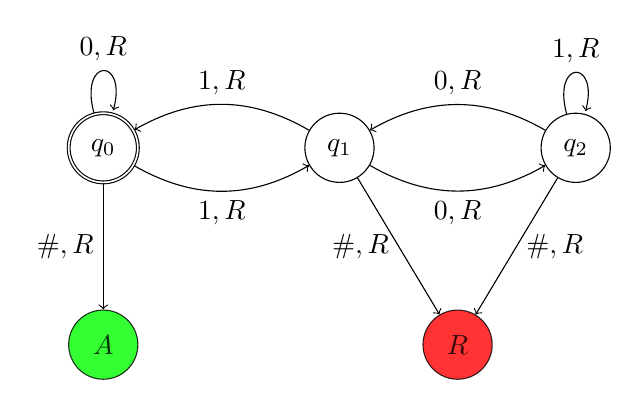
\begin{tikzpicture}
                \node[state, accepting] (q0) at (0, 0) {$q_0$};
                \node[state] (q1) at (3, 0) {$q_1$};
                \node[state] (q2) at (6, 0) {$q_2$};
                \node[state, fill=green, opacity=0.8] (A) at (0, -2.5) {$A$};
                \node[state, fill=red, opacity=0.8] (R) at (4.5, -2.5) {$R$};
    
                \draw[->] (q0) edge[loop above] node {$0, R$} (q0);
                \draw[->] (q0) edge[bend right] node[below] {$1, R$} (q1);
                \draw[->] (q1) edge[bend right] node[above] {$1, R$} (q0);
                \draw[->] (q1) edge[bend right] node[below] {$0, R$} (q2);
                \draw[->] (q2) edge[bend right] node[above] {$0, R$} (q1);
                \draw[->] (q2) edge[loop above] node {$1, R$} (q2);
                \draw[->] (q0) edge node[left] {$\#, R$} (A);
                \draw[->] (q1) edge node[left] {$\#, R$} (R);
                \draw[->] (q2) edge node[right] {$\#, R$} (R);
            \end{tikzpicture}
        \end{figure}
        You are given a basic representation of this FSM as code in Teams.
%         The following is a program representation for the FSM:
% \begin{lstlisting}[language=TML]
% alphabet = {0, 1}
% module q0 {
%     if 0 {
%         move right
%     } if 1 {
%         move right
%         goto q1
%     } if blank {
%         move right
%         accept
%     }
% }
% module q1 {
%     if 1 {
%         move right
%         goto q0
%     } if 
% }
% \end{lstlisting}
        \begin{enumerate}
            \item Does the TM accept the values:
            \begin{enumerate}
                \item $2 = 10$
                \begin{solution}
                    
                \end{solution}
                
                \item $1 = 1$
                \begin{solution}
                    
                \end{solution}
                
                \item $6 = 100$
                \begin{solution}
                    
                \end{solution}
                
                \item $5 = 101$
                \begin{solution}
                    
                \end{solution}
                
                \item $8 = 110$
                \begin{solution}
                    
                \end{solution}
            \end{enumerate}
            
            \item Describe the values this program accepts.
            \begin{solution}
                % IsDiv3
            \end{solution}
        \end{enumerate} 
        \newpage   
        
        \item Consider the following TM FSM:
        \begin{figure}[H]
            \centering
            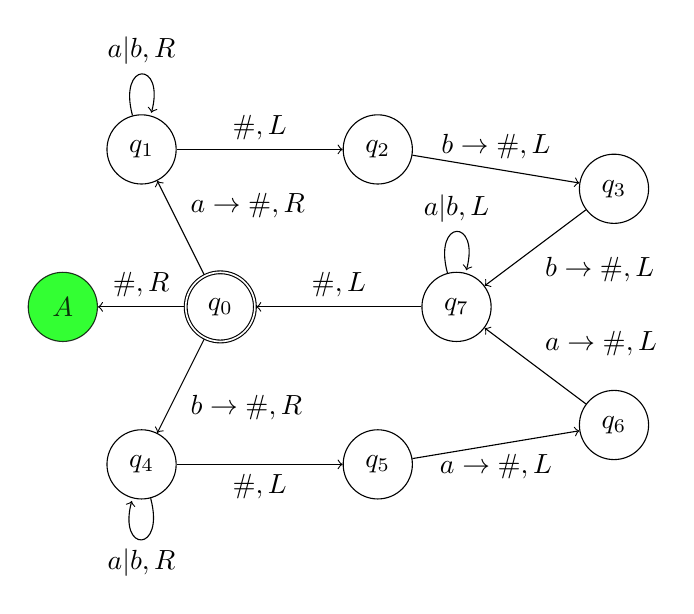
\begin{tikzpicture}
                \node[state, accepting] (q0) at (3, 0) {$q_0$};
                \node[state] (q1) at (2, 2) {$q_1$};
                \node[state] (q2) at (5, 2) {$q_2$};
                \node[state] (q3) at (8, 1.5) {$q_3$};
                \node[state] (q4) at (2, -2) {$q_4$};
                \node[state] (q5) at (5, -2) {$q_5$};
                \node[state] (q6) at (8, -1.5) {$q_6$};
                \node[state] (q7) at (6, 0) {$q_7$};
                \node[state, fill=green, opacity=0.8] (A) at (1, 0) {$A$};
    
                \draw[->] (q0) -- node[above right] {$a \to \#, R$} (q1);
                \draw[->] (q0) -- node[below right] {$b \to \#, R$} (q4);
                \draw[->] (q0) -- node[above] {$\#, R$} (A);
                \draw[->] (q1) edge[loop above] node {$a|b, R$} (q1);
                \draw[->] (q1) -- node[above] {$\#, L$} (q2);
                \draw[->] (q2) -- node[above] {$b \to \#, L$} (q3);
                \draw[->] (q3) -- node[below right] {$b \to \#, L$} (q7);
                \draw[->] (q4) edge[loop below] node {$a|b, R$} (q4);
                \draw[->] (q4) -- node[below] {$\#, L$} (q5);
                \draw[->] (q5) -- node[below] {$a \to \#, L$} (q6);
                \draw[->] (q6) -- node[above right] {$a \to \#, L$} (q7);
                \draw[->] (q7) edge[loop above] node {$a|b, L$} (q7);
                \draw[->] (q7) -- node[above] {$\#, L$} (q0);
            \end{tikzpicture}
        \end{figure}
        % Checks 
        NOTE: The missing transitions go to the reject state, i.e. $q_2$, $q_3$ to $a|\#$ and $q_5$, $q_6$ to $b|\#$ are rejected. You are given a basic representation of this FSM as code in Teams.
        \begin{enumerate}
            \item Does this TM accept the values:
            \begin{enumerate}
                \item $ab$
                \begin{solution}
                    
                \end{solution}

                \item $abb$
                \begin{solution}
                    
                \end{solution}

                \item $aabb$
                \begin{solution}
                    
                \end{solution}
                
                \item $bbaaaa$
                \begin{solution}
                    
                \end{solution}

                \item $abba$
                \begin{solution}
                    
                \end{solution}

                \item $abab$
                \begin{solution}
                    
                \end{solution}
            \end{enumerate}

            \item Describe the values this program accepts.
            \begin{solution}
                
            \end{solution}
        \end{enumerate}
    \end{enumerate}
    % Checks isDiv4
    
    % NOTE: The missing links go to the reject state, 
    
% // accepts strings of the form a^n b^n c^n
% alphabet = {a, b, c}
% module aNbNcN {
%     if blank {
%         accept
%     } if c {
%         reject
%     } 
%     // a => remove a, go to the end, replace c with a
%     if a {
%         move right
%         // move to the end
%         while a, b, c {
%             move right
%         } if blank {
%             move left
%             // go past the a's and then replace the last c with an a
%             while a {
%                 move left
%             } if blank, b {
%                 reject
%             } if c {
%                 changeto a
%                 move left
%                 // go to the start
%                 while a, b, c {
%                     move left
%                 } if blank {
%                     move right
%                     goto aNbNcN
%                 }
%             }
%         }
%     } if b {
%         goto bNaN
%     }
% }
% module bNaN {
%     if blank {
%         accept
%     } if a, c {
%         reject
%     } if b {
%         changeto blank
%         move right
%         // go to the end (c is a direct reject)
%         while a, b {
%             move right
%         } if c {
%             reject
%         } if blank {
%             move left
%             // remove the a and move to the start
%             if b, c, blank {
%                 reject
%             } if a {
%                 changeto blank
%                 while a, b {
%                     move left
%                 } if c {
%                     reject
%                 } if blank {
%                     goto bNaN
%                 }
%             }
%         }
%     }
% }
    
    
    
\end{document}
